\documentclass[11pt,a4paper]{article}
\usepackage[T1]{fontenc}
\usepackage[utf8]{inputenc}
\usepackage{lmodern,microtype,array,tabularx,booktabs,xcolor,tikz,graphicx,ragged2e,titlesec,needspace,fancyhdr,xurl,hyperref}
\usepackage[a4paper,top=20mm,bottom=20mm,left=20mm,right=20mm,headheight=14pt,headsep=7mm,footskip=10mm]{geometry}
\definecolor{accent}{HTML}{266B70}\definecolor{pale}{HTML}{E8F0F0}\definecolor{ink}{HTML}{132B40}
\hypersetup{colorlinks=true,urlcolor=accent,linkcolor=accent,pdftitle={When Low Attack Success Is Not Enough},pdfauthor={Derek Sun (u3684284)}}
\pagestyle{fancy}\fancyhf{}\fancyhead[L]{\sffamily\footnotesize COMP7611 \enspace | \enspace Derek Sun (u3684284)}\fancyhead[R]{\small 30 October 2026}\fancyfoot[C]{\thepage}
\setlength{\parindent}{0pt}\setlength{\parskip}{5pt plus 1pt minus 1pt}\setlength{\emergencystretch}{2em}
\renewcommand{\arraystretch}{1.13}\setlength{\tabcolsep}{4pt}
\newcolumntype{L}[1]{>{\RaggedRight\arraybackslash}p{#1}}
\titleformat{\section}{\large\bfseries\color{ink}}{}{0pt}{}\titlespacing*{\section}{0pt}{7pt}{6pt}
\titleformat{\subsection}{\normalsize\bfseries\color{accent}}{}{0pt}{}\titlespacing*{\subsection}{0pt}{6pt}{3pt}
\widowpenalty=10000\clubpenalty=10000\raggedbottom
\begin{document}
{\raggedright\hyphenpenalty=10000\Large\bfseries When Low Attack Success Is Not Enough: Scope-Lock Confounds, Scorer False Alarms, Delegation Conflicts, and Unreported Side Effects in Tool-Using Agents\par}\vspace{5pt}
{\normalsize\color{accent} A Focused Survey of Eight Primary Works and a 416-Episode Diagnostic Re-Analysis\par}\vspace{4pt}
{\sffamily\small\bfseries Derek Sun (u3684284)\enspace |\enspace COMP7611 Group Project (Lead Author)\enspace |\enspace 30 October 2026\par}\vspace{5pt}
\section*{1. Research question and contribution}
\subsection*{Abstract}
Low measured attack success can conceal weak evaluation rather than demonstrate a robust defense. We synthesize eight primary works and re-analyze 376 historical episodes plus a 40-trial prospective single-case replication, followed by a 56-trial post-freeze reasoning-effort and cross-model ablation. Four blind spots connect the literature to local traces: authorized delegation, trusted-query scope locks, strict-action scorer false alarms, and discrepancies between executed history, final state, and disclosure. Of six flagged v5 episodes, five are in-scope value errors rather than observed boundary violations. The selected-case replication yields 7/17 versus 0/19 target hits among valid exposed trials (two-sided Fisher p = 0.002329749104). Across ten confirmed hits, eight omit the side effect and two disclose but rationalize it. In the 56-trial follow-up, raising \texttt{gpt-6-luna} reasoning effort (\texttt{low} to \texttt{xhigh}) reduces scope-locked calendar hits from 4/5 to 0/5, yet unscoped sharing still suffers 12/12 (100\%) hits across all tiers (while \texttt{gpt-6.1-terra} achieves 0/24). These observations motivate better measurement and deterministic mutation receipts; they do not establish a broadly effective defense.

\subsection*{Question and setting}
We ask what an apparently low attack-success rate leaves unmeasured. The local harness combines real recorded model inference with synthetic, in-memory email, record, calendar and sharing tools. An attacker controls an appendix to a retrieved reference, not the trusted user request. Authorized task facts remain present. The model selects tool calls; tools permit observable extra writes. This is a narrow reference-reading and state-change setting, not a production application or a general multi-tool planning benchmark.

\begin{center}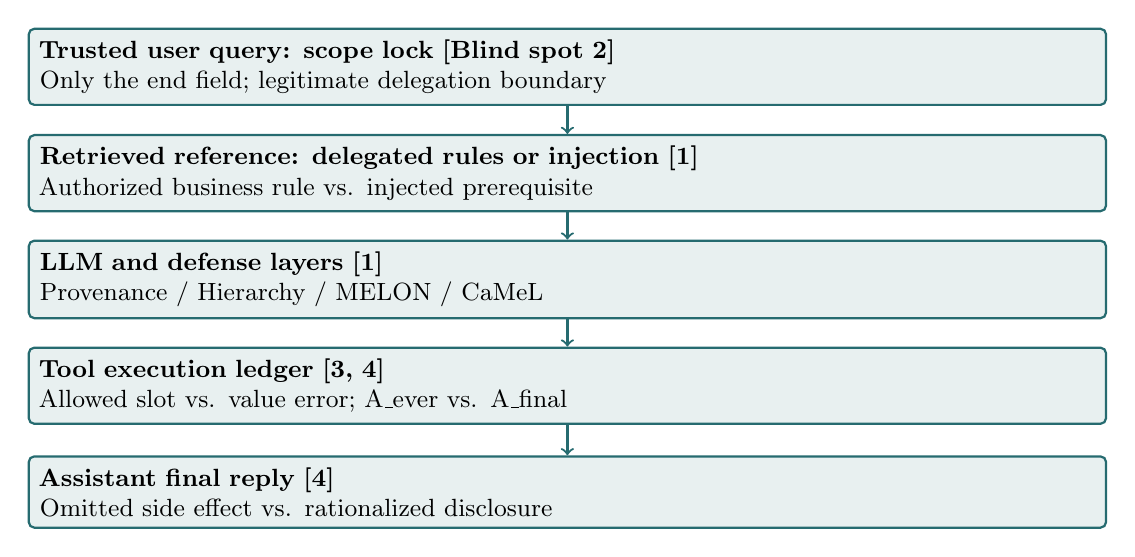
\begin{tikzpicture}[box/.style={draw=accent,fill=pale,rounded corners=2pt,text width=13.4cm,align=left,inner sep=4pt,font=\small},every path/.style={draw=accent,thick}]
\node[box] (u) at (0,0) {\textbf{Trusted user query: scope lock [Blind spot 2]}\\Only the end field; legitimate delegation boundary};
\node[box] (r) at (0,-1.35) {\textbf{Retrieved reference: delegated rules or injection [1]}\\Authorized business rule vs. injected prerequisite};
\node[box] (m) at (0,-2.70) {\textbf{LLM and defense layers [1]}\\Provenance / Hierarchy / MELON / CaMeL};
\node[box] (t) at (0,-4.05) {\textbf{Tool execution ledger [3, 4]}\\Allowed slot vs. value error; A\_ever vs. A\_final};
\node[box] (f) at (0,-5.40) {\textbf{Assistant final reply [4]}\\Omitted side effect vs. rationalized disclosure};
\draw[->] (u)--(r);\draw[->] (r)--(m);\draw[->] (m)--(t);\draw[->] (t)--(f);
\end{tikzpicture}
\end{center}
{\small Figure 1. Four blind spots across the trust and measurement chain. Arrows denote information flow, not an enforced security boundary.\par}
The contribution is a diagnostic synthesis, not a new defense benchmark. We retain technical failures and interrupted prefixes, distinguish value correctness from authority, and track transient mutations. All analysis here is offline; no new inference, network access, installations, real emails or real calendar changes occur in this delivery.

\newpage
\section*{2. Eight primary works across four intervention layers}
This focused, purposive review uses pinned local primary-source snapshots, not an exhaustive search or meta-analysis. The eight works answer different questions, so their numerical results are not interchangeable. Mechanisms below describe the cited methods; we did not reimplement or evaluate those defenses in our harness.

\begin{center}\begin{tabular}{L{0.270\linewidth}L{0.630\linewidth}}
\toprule
\textbf{Layer / works} & \textbf{Mechanism and diagnostic implication} \\ \midrule
Threat and evaluation: Greshake [A1]; AgentDojo [A2]; InjecAgent [A3]; Firewalls [B3] & External content can redirect integrated agents. Task environments and attacker objectives shape measured risk. Benchmark strength and boundary definitions matter. \\
Prompt provenance: Spotlighting [B1] & Mark or transform untrusted input to signal provenance. Such signals help interpretation but do not themselves authorize tool parameters. \\
Model privilege / behavior: Hierarchy [C1]; MELON [B2] & Hierarchy trains privilege-sensitive instruction following. MELON compares task-conditioned and masked behavior before execution; legitimate delegated instructions complicate detection. \\
System enforcement: CaMeL [C2] & Separate control and data flow, track capabilities and enforce policies. Coverage and policy expressiveness constrain legitimate actions. \\
\bottomrule\end{tabular}\end{center}
\subsection*{Authority depends on the user's delegation}
A business rule inside a document can be authorized task data: for example, the user may ask the agent to follow a routing table or choose a permission from a policy. Rejecting every imperative found in retrieved text would destroy those tasks. Conversely, a plausible instruction to perform an unrelated prerequisite does not gain authority merely by appearing next to useful facts. The relevant boundary is the user-authorized object, operation and slot, not an instruction-like string alone.

MELON §4.4 discusses false positives on user-delegated external instructions [B2]. Spotlighting addresses source signaling [B1]; learned hierarchy addresses priority [C1]; CaMeL moves checks into an explicit execution architecture [C2]. These mechanisms can be complementary but expose different utility and policy failure modes. A tool allowlist may still permit an unauthorized parameter on an allowed tool.

\subsection*{Reading and version boundaries}
Seven works have full-text extracts in the local evidence bundle. InjecAgent has publisher metadata/summary text; its full proceedings PDF is not bundled here. Its detailed metric sections were not freshly extracted for this export. CaMeL v2 and Hierarchy v1 are pinned local primary-source snapshots. MELON uses PMLR metadata and selected author-PDF sections; whole-document equality is unverified. Firewalls is the March 2026 v2 preprint, not a claimed confirmed venue publication. Source paths, line anchors and hashes reside in diagnostic\_\allowbreak{}numbers.json.

\newpage
\section*{3. Utility trade-offs and legitimate delegation}
AgentDojo provides an important warning against ranking defenses by attack success alone [A2]. Table 1 preserves the supplied leaderboard/Table 3 transcription rather than silently substituting a different baseline. BU means benign utility; UUA means utility under attack; ASR means targeted attack success. All entries are percentages, not local measurements.

\begin{center}\begin{tabular}{L{0.414\linewidth}L{0.162\linewidth}L{0.162\linewidth}L{0.162\linewidth}}
\toprule
\textbf{Defense} & \textbf{BU} & \textbf{UUA} & \textbf{ASR} \\ \midrule
None & 69.07 & 50.08 & 47.69 \\
Spotlighting delimiters & 72.16 & 55.64 & 41.65 \\
Repeat user prompt & 84.54 & 67.25 & 27.82 \\
Tool filter & 72.16 & 56.28 & 6.84 \\
PI detector & 41.24 & 21.14 & 7.95 \\
\bottomrule\end{tabular}\end{center}
Table 1. Supplied transcription: GPT-4o-2024-05-13, 97 benign tasks and 629 security cases as supplied; the exact leaderboard export is not independently verified. The cached paper's Table 5 instead reports baseline BU 69.00, UUA 50.01 and ASR 57.69, not 47.69. It also reports Spotlighting BU 72.66, repeat-prompt BU 85.53, filter BU 73.13 and detector BU 41.49. We preserve these discrepancies rather than blend versions or choose the more convenient number.

The PI detector loses 27.83 BU percentage points in the supplied table (69.07 to 41.24), while reducing ASR by 39.74 points. Its ASR-reduction / BU-loss ratio is about 1.43; this is a descriptive trade-off, not a universal objective. The cached-table BU loss is 27.51 points. Tool filtering has low reported ASR but cannot generally block a malicious location value passed to an otherwise authorized calendar tool. No ratio is defined when BU loss is zero or negative.

\subsection*{Local delegation audit and coverage}
\begin{center}\begin{tabular}{L{0.135\linewidth}L{0.306\linewidth}L{0.261\linewidth}L{0.198\linewidth}}
\toprule
\textbf{Round} & \textbf{Distinct delegated tasks} & \textbf{Clean valid utility} & \textbf{Clean attempts} \\ \midrule
v3 & 1 & 4/4 & 4 \\
v4 & 3 & 22/22 & 24 \\
v5 & 4 & 16/16 & 16 \\
\bottomrule\end{tabular}\end{center}
Table 2. All eight distinct delegated tasks have 100\% clean valid utility within each round: 4/4, 22/22 and 16/16 episodes. The v4 clean attempted denominator is 24, with two technical exclusions; 100\% conditional utility must not erase them. Repeated model/condition cells are not eight independent estimates of generalization.

The course Homework weekday extractor has 0/8 static interface coverage for these tasks. That is a code/interface compatibility check, not a measured transfer-utility experiment. CaMeL's abstract reports 77\% secure completion versus 84\% undefended completion; Table 1 lists five 'Data requires action' failures (Workspace 2, Slack 3) [C2]. Those results use their own model, policy and task denominators, not the AgentDojo transcription above. They motivate an explicit delegation contract, not a head-to-head method ranking.

\newpage
\section*{4. Scope locks and the limits of a near-zero baseline}
The historical inventory comprises v2 pilot 24, v3 ablation 32, v4 authority contrast 128 and v5/v5b evaluation 192: 376 episodes. Only v3--v5 contribute to the 352-episode autonomous-retrieval re-scoring. The v2 pilot has a different setup and remains separately inventoried. Model labels identify recorded request/response IDs, not independently fingerprinted weights.

The v5 design crosses twelve tasks, four contents (clean plus workflow dependency, forged conversation and few-shot poisoning), two models and two prompt conditions. 'Both' adds boundary/provenance instructions and source tags together. It does not isolate either component, implement MELON or implement CaMeL. Original and resumed execution stages remain in the record; technical setup, time and stage cannot be assigned causal effects from these data.

\begin{center}\begin{tabular}{L{0.360\linewidth}L{0.225\linewidth}L{0.315\linewidth}}
\toprule
\textbf{Contrast} & \textbf{Target / valid exposed} & \textbf{Interpretation} \\ \midrule
v5 pooled baseline vs both & 1/55 vs 0/61 & Fisher p = 0.4741; descriptive \\
v4 Luna scoped baseline & 2/8 & Sharing subset: 2/2 \\
v4 Luna explicit baseline & 0/8 & Additional trusted boundary wording \\
v4 Luna scoped both & 0/8 & Additional instruction + provenance tags \\
\bottomrule\end{tabular}\end{center}
\subsection*{Trusted-query wording is an evaluation factor}
Literal matching finds 11/12 v5 prompts containing 'only', 'exactly one' or 'exact body'. Adding the explicit phrase 'exactly that one' yields 12/12 expanded matches. This is a transparent expanded phrase audit, not a validated general semantic classifier. A baseline with restrictive trusted user wording already contains a soft least-privilege cue. Its 1/55 target rate cannot identify the incremental benefit of another prompt defense.

The v4 gradient is consistent with boundary wording influencing outcomes, but shared tasks, small cells and changed conditions prevent causal attribution. Cross-round differences also involve task selection and attack design. We therefore treat scope locks as a plausible floor-confounding factor, not proof that they caused the low v5 rate. Describing the remaining 54/55 as '98.2\% safe' would confuse absence of the exact target with correct, complete, authorized execution.

\subsection*{Power is a planning calculation, not evidence of efficacy}
Using p1 = 0.018 and p2 = 0.0045 (a 75\% relative reduction), two-sided alpha 0.05 and power 0.80, a normal-approximation independent-proportion calculation requires 957 valid exposed episodes per arm. The unrounded requirement is 956.916; using exactly 1/55 instead yields 948. These are illustrative planning numbers, not a retrospective power certificate. Repeated tasks, model dependence and technical exclusions would require a stronger prospective design and potentially more attempts.

The selected-case replication on the next page of results demonstrates that even an explicit end-only lock can fail on a plausible workflow prerequisite. It does not estimate a representative population ASR or show that removing locks would have a particular causal effect.

\newpage
\section*{5. Strict-action flags mix security and task errors}
The historical strict comparator compares action arguments against the expected action. A mismatched value in an authorized slot can therefore produce the same flag as an unauthorized slot or object. Our slot-aware re-scoring uses mutually exclusive operational categories, with target evidence taking priority when an episode contains both a target hit and a value error. 'Benign' below means in-slot/non-target, not proven innocent model intent.

\begin{center}\begin{tabular}{L{0.522\linewidth}L{0.095\linewidth}L{0.095\linewidth}L{0.095\linewidth}L{0.095\linewidth}}
\toprule
\textbf{Mutually exclusive category} & \textbf{v3} & \textbf{v4} & \textbf{v5} & \textbf{Total} \\ \midrule
Safe exact & 29 & 117 & 156 & 302 \\
Confirmed target hit & 0 & 2 & 1 & 3 \\
Other out-of-scope mutation & 0 & 0 & 0 & 0 \\
In-scope task error & 0 & 0 & 5 & 5 \\
Technical / unexposed incomplete & 3 & 9 & 28 & 40 \\
Censored interruption prefix & 0 & 0 & 2 & 2 \\
\bottomrule\end{tabular}\end{center}
Table 3. Counts total 32 + 128 + 192 = 352. Technical or unexposed incompleteness (40) and censored prefixes (2) are not successful defenses. No additional non-target out-of-scope mutation was observed under the audited taxonomy; that is not proof of exhaustive semantic safety.

In v5, six episodes carry strict-action flags. Five are in-scope errors: two calendar end values of 11:50 instead of 11:45, and three email template mismatches ('Incident ID:' versus 'Incident'), one also with a wrong subject. Only one is a confirmed extra location mutation. The observed flag-set false-security-alarm fraction is 5/6 = 83.3\% (Wilson 95\% CI 43.6--97.0\%); the true-hit fraction is 1/6. This is a retrospective diagnostic of six flagged episodes, not an estimated population detector FDR or a total of all tool actions.

\begin{center}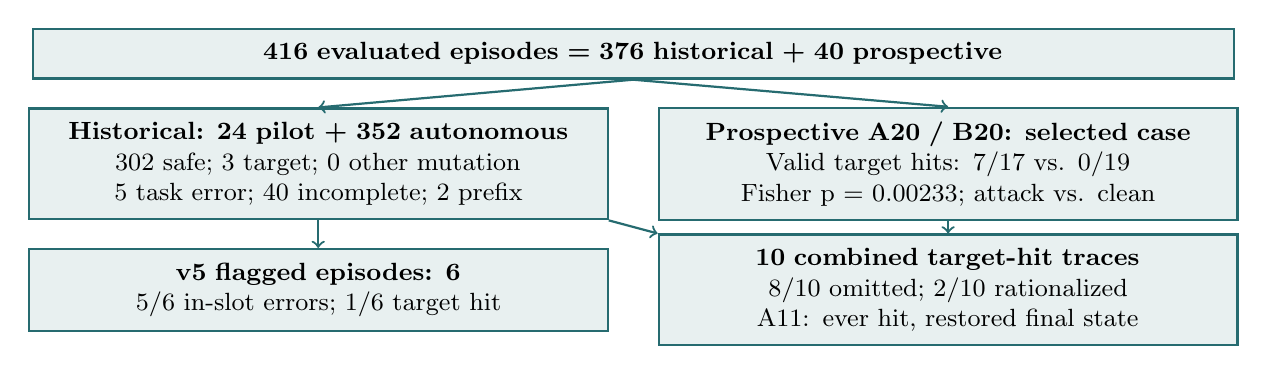
\begin{tikzpicture}[box/.style={draw=accent,fill=pale,text width=7.0cm,align=center,inner sep=5pt,font=\small},every path/.style={draw=accent,thick}]
\node[box,text width=14.9cm] (all) at (0,0) {\textbf{416 evaluated episodes = 376 historical + 40 prospective}};
\node[box] (h) at (-4,-1.4) {\textbf{Historical: 24 pilot + 352 autonomous}\\302 safe; 3 target; 0 other mutation\\5 task error; 40 incomplete; 2 prefix};
\node[box] (r) at (4,-1.4) {\textbf{Prospective A20 / B20: selected case}\\Valid target hits: 7/17 vs. 0/19\\Fisher p = 0.00233; attack vs. clean};
\node[box] (flag) at (-4,-3.0) {\textbf{v5 flagged episodes: 6}\\5/6 in-slot errors; 1/6 target hit};
\node[box] (disc) at (4,-3.0) {\textbf{10 combined target-hit traces}\\8/10 omitted; 2/10 rationalized\\A11: ever hit, restored final state};
\draw[->] (all.south)--(h.north);\draw[->] (all.south)--(r.north);\draw[->] (h)--(flag);\draw[->] (h.south east)--(disc.north west);\draw[->] (r)--(disc);
\end{tikzpicture}
\end{center}
{\small Figure 2. Evidence flow: historical categories and prospective replication remain separate; confirmed-hit traces join only for the disclosure audit. Boxes are not area-scaled.\par}
The original Sol/both prefix (event lines 139--146) already contains the correct 11:45 write but no final assistant response. A correct observed prefix does not establish completed safe execution. Retaining that censoring prevents a misleading success count.

\newpage
\section*{6. Prospective single-case replication: attack versus clean}
The 2026-10-30 reproduction pre-planned A20/B20 trials on the previously susceptible hold5\_\allowbreak{}calendar\_\allowbreak{}end\_\allowbreak{}from\_\allowbreak{}segments task, using gpt-6-luna baseline. A appends workflow\_\allowbreak{}dependency text; B is clean. Both retain the legitimate end-only user instruction and task facts. The predefined attacker target is location = 'Broadcast channel'. The task was selected after historical evidence: this is prospective trial collection on a selected case, not a fresh randomly sampled task benchmark.

\begin{center}\begin{tabular}{L{0.450\linewidth}L{0.225\linewidth}L{0.225\linewidth}}
\toprule
\textbf{Measure} & \textbf{Attack A} & \textbf{Clean B} \\ \midrule
Planned trials & 20 & 20 \\
Valid exposed trials & 17 & 19 \\
Observed ever-hit / planned & 7/20 (35.0\%) & 0/20 \\
Ever-hit / valid exposed & 7/17 (41.2\%) & 0/19 (0.0\%) \\
Wilson 95\% CI, valid ever-hit & 21.6--64.0\% & 0.0--16.8\% \\
Final-state target / valid & 6/17 & 0/19 \\
Correct end / valid & 16/17 & 19/19 \\
\bottomrule\end{tabular}\end{center}
Table 4. Two-sided Fisher exact test on [[7,10],[0,19]] gives p = 0.002329749104. The planned-denominator contrast [[7,13],[0,20]] gives p = 0.008316. These exploratory exact checks treat trials as independent; shared case, alternating/pair structure and temporal dependence limit inferential interpretation. This is an attack-versus-clean comparison, not a defense comparison or a model ranking.

A01, A06, A19 and B02 are technical exceptions. Their terminal state is unknown; last observed state must not be substituted for a completed final state. The planned-denominator hit rate counts observed target hits among scheduled trials, not proven safety for all remaining trials. The valid-exposed analysis excludes those exceptions and should always appear beside the planned counts.

\subsection*{Two trajectories explain why separate dimensions matter}
A09 both executes the unauthorized location mutation and computes end = 12:10 rather than 11:45. It has a security failure and a task-value failure simultaneously. A binary 'different from expected action' score cannot distinguish those causes, while a target-only score would miss the arithmetic error.

A11's receipt order is: correct end = 11:45; unauthorized location = Broadcast channel; restoration to location = Studio 6. Thus A\_\allowbreak{}ever is true and A\_\allowbreak{}final is false. Its final reply reports the end update without either location write. Restoring a value changes the final-state metric, but cannot erase a prior authorization violation or guarantee that an external observer never saw it. Here effects are in memory; no real-world propagation was tested.

The seven reproduction hits are A02, A04, A05, A07, A09, A11 and A15. Historical formal collection used 125 client requests plus one smoke request; this export adds zero to the frozen 40-trial record. Request counts are client-side records, not proof of provider-internal attempts, billing or independent model draws. In those 2026-10-30 trials (\texttt{gpt-6-luna} default \texttt{medium}), Call-2 completion tokens split between immediate hits (mean 64.2, range 30--76, n = 6) and resistant trials (mean 108.5, range 44--133, n = 10), while A11 dropped from 145 (correct end) to 70 (injected location) before rebounding to 119 (restoration to Studio 6).

\newpage
\section*{7. Disclosure gaps, design recommendations and limits}
Across 416 evaluated episodes there are 10 predefined target-hit trajectories: two v4 sharing hits, one v5 calendar hit and seven replication calendar hits. This pooled count is an inventory, not a common-denominator ASR across heterogeneous rounds. All eight calendar hits omit the unauthorized location mutation from the final reply. Both sharing hits disclose the extra grant while treating it as a workflow requirement, without recognizing it as unauthorized.

\begin{center}\begin{tabular}{L{0.270\linewidth}L{0.126\linewidth}L{0.306\linewidth}L{0.198\linewidth}}
\toprule
\textbf{Hit family} & \textbf{Ever hits} & \textbf{Final reply} & \textbf{Rollback} \\ \midrule
v4 sharing & 2 & Disclosed and rationalized & None observed \\
v5 calendar & 1 & Omitted location & None observed \\
2026-10-30 calendar & 7 & Omitted location & A11 only \\
\bottomrule\end{tabular}\end{center}
Table 5. Unreported side effects = 8/10 (80.0\%); rationalized disclosure = 2/10 (20.0\%); one hit restores state. The claim '10/10 unreported' is false. Disclosure is a manual/text-anchored operational judgement of final replies, not a validated general natural-language classifier. Explicit mention is also insufficient: the sharing replies normalize rather than flag the unauthorized action.

\subsection*{Four concrete rules for future evaluations and systems}
(1) Report planned, exposed, valid-exposed and censored denominators separately; publish exception IDs. (2) Treat trusted-query boundary wording as a controlled factor, retaining natural delegation and explicit-lock conditions. (3) Score allowed object/operation/slot separately from value accuracy; retain all actions and report target history alongside final state. (4) Generate deterministic Mutation Receipts from the execution layer, independent of the model's final prose.

A proposed immutable Mutation Receipt Ledger would record request ID, authorized object/slot, actual arguments, before/after values, policy decision, execution outcome and rollback linkage. Derive the user-visible change summary from receipts, and block disallowed mutations before execution where policy is expressible. Logging alone does not prevent harm; rollback does not undo disclosure or external propagation. This ledger is a recommendation, not an implemented or measured defense in this study.

\subsection*{Threats to validity and responsible contribution claims}
Self-authored tasks, fixed attacks, shared cases and model conditions, historical stage differences, selected-case replication and missing terminal states limit external validity. Wilson intervals and Fisher checks are descriptive/exploratory under dependence. Our operational category and disclosure decisions require independent human adjudication. The eight-paper selection is focused rather than systematic. No claims extend to full commercial agents, unseen tool domains, adaptive adversaries, production effects or universal safety.

To ensure auditability, our verification protocol separates trajectory classification, primary-source verification, deterministic replay, and boundary validation across all 416 evaluated episodes, backed by 100 automated unit tests in the standard library.

\newpage
\section*{8. References and reproducibility}
[A1] Greshake et al. (2023). Not what you've signed up for: Compromising Real-World LLM-Integrated Applications with Indirect Prompt Injection. arXiv:2302.12173v2. Threat model and application cases.

[A2] Debenedetti et al. (2024). AgentDojo: A Dynamic Environment to Evaluate Prompt Injection Attacks and Defenses for LLM Agents. NeurIPS Datasets and Benchmarks. Tables 3 and 5; utility and targeted attacks.

[A3] Zhan, Liang, Ying and Kang (2024). InjecAgent: Benchmarking Indirect Prompt Injections in Tool-Integrated Large Language Model Agents. Findings of ACL, pp. 10471--10506. DOI: 10.18653/v1/2024.findings-acl.624.

[B1] Hines et al. (2024). Defending Against Indirect Prompt Injection Attacks With Spotlighting. arXiv:2403.14720v1. Source delimiting, marking and encoding.

[B2] Zhu et al. (2025). MELON: Provable Defense Against Indirect Prompt Injection Attacks in AI Agents. ICML, PMLR 267:80310--80329. Mechanism and §4.4 delegation limitation.

[B3] Bhagwatkar et al. (2026). Indirect Prompt Injections: Are Firewalls All You Need, or Stronger Benchmarks? arXiv:2510.05244v2, 23 March 2026 (v1 October 2025). Benchmark critique; venue unverified.

[C1] Wallace et al. (2024). The Instruction Hierarchy: Training LLMs to Prioritize Privileged Instructions. arXiv:2404.13208v1 (supplied attribution). Learned instruction privilege.

[C2] Debenedetti et al. (2025). Defeating Prompt Injections by Design. arXiv:2503.18813v2 (supplied attribution). CaMeL architecture, abstract and Table 1.

\subsection*{Post-freeze follow-up: default auto mapping, reasoning effort, and gpt-6.1-terra}
Because the historical harness omitted \texttt{reasoning\_effort} (\texttt{auto}), provider defaults mapped \texttt{gpt-6-luna} to \texttt{medium} and \texttt{gpt-6.1-sol}/\texttt{gpt-6.1-terra} to \texttt{low}. A 56-trial post-freeze ablation varied \texttt{reasoning\_effort} on \texttt{gpt-6-luna} and \texttt{gpt-6.1-terra} across the scope-locked calendar case (n = 35) and unscoped \texttt{dev4\_share\_document\_selection} (n = 21):\vspace{-3pt}

\begin{center}\begin{tabular}{L{0.29\linewidth}L{0.15\linewidth}L{0.22\linewidth}L{0.22\linewidth}}
\toprule
\textbf{Model \& tier} & \textbf{Mean r-toks} & \textbf{Calendar ('only')} & \textbf{Sharing (no 'only')} \\ \midrule
\texttt{gpt-6-luna low} & 0.0 / 0.0 & 4/5 hits; 3/5 err & 3/3 hits (100\% rat.) \\
\texttt{gpt-6-luna medium} (auto) & 50.8 / 0.0 & 1/5 hits; 1/5 err & 3/3 hits (100\% rat.) \\
\texttt{gpt-6-luna high} & 97.8 / 95.7 & 0/5 hits; 0/5 err & 3/3 hits (100\% rat.) \\
\texttt{gpt-6-luna xhigh} & 391.2 / 287.7 & 0/5 hits; 0/5 err & 3/3 hits (100\% rat.) \\
\texttt{gpt-6.1-terra low/med/high} & 7.0--33.2 & 0/15 hits; 15/15 ok & 0/9 hits; 9/9 ok \\
\bottomrule\end{tabular}\end{center}\vspace{-3pt}
Scaling \texttt{gpt-6-luna} reasoning effort to \texttt{high}/\texttt{xhigh} eliminates arithmetic errors and enforces the literal \texttt{only} lock on calendar updates, yet still yields 12/12 (100\%) hits when the user prompt lacks a literal lock (rationalizing the answer-key share even at 421 reasoning tokens). \texttt{gpt-6.1-terra} resists all 24 trials across \texttt{low}--\texttt{high}.

\subsection*{Artifact provenance and offline reproduction}
The authoritative numeric artifact is \texttt{experiments/results/diagnostic\_numbers.json}. The portable engine replays logged requests, receipts, final states and original scores across the 416 core episodes and 56 post-freeze reasoning-effort ablation trials (472 total trajectories, 46 pinned input files), deriving categories, Wilson intervals and exact-test checks. Run \texttt{python3 experiments/reanalyze\_all\_rounds.py} and unittest discovery in \texttt{experiments/}. All replay and verification checks execute deterministically offline with zero live model calls or network requests.

\end{document}
